\documentclass[12pt, letterpaper]{article}

\usepackage[hyphens,spaces,obeyspaces]{url}
\usepackage{graphicx}
\usepackage[margin=1in]{geometry}
\usepackage{seqsplit}
\graphicspath{ {./images/} }
    

\title{CMPUT 499 Final Paper}
\author{Monica Bui}

\begin{document}

\begin{titlepage}
    \centering
    \large
    \vspace{1cm}
    Exploring Software Library Metrics \\ 
    with Repository Badges \\
    \vspace{1cm}
    by \\
    \vspace{1cm}
    Monica Bui \\
    University of Alberta \\
    bui1@ualberta.ca \\
    \vspace{1cm}
    Sarah Nadi \\
    University of Alberta \\
    nadi@ualberta.ca \\
    \vspace{10cm}
    Scripts \& Documentation: \\
    https://github.com/ualberta-smr/bui-course-f18
\end{titlepage}

\tableofcontents

\listoffigures
\newpage

\section{Introduction} 
% How do developers select libraries
% Iinstead of using websites, and online sources
% we look to create badges that can be shown on the spot to users
% to help them seee metrics and pick the best library

Libraries, Frameworks, and Application Programming Interfaces (APIs) provide developers a way to reuse existing functionalities
built by someone else without having to re-implement already built features. Given a large collection of libraries out there,
it is often difficult and not clear how to select the best one to use for your own project. 


Developers may resort to first doing a general search of their desired library features with search results indicating
various resources such as a Q\&A website like StackOverflow \cite{stackoverflow} or a website that hosts open source libraries such as Github \cite{github}.


Previous research has examined different, inner aspects of libraries that may have mentioned in the above
online resources \cite{githubbadges,apiwave,metrics,opinerarticle,analogical}. These aspects or defined 


Based on Trockman's et al. \cite{githubbadges} badge recommendations, we look to create 
dynamic badges that take more work to create i.e assessment badges, metric itself is quantifiable, and
we implement badges that do not exist yet so we do not develop already existing badges.
These suggestions will be helpful to produce effective, reliable
badges that developers can use for their projects and help them select libraries to use.

% dont explicity reccomend libraries. Allow develoeprs to make their
% own judgement to select librarie. Another quanittiative tool
% to help compare b/w 

\section{Related Work}
\subsection{Library Selection Methods}
% This work focused on explicity recomending libraries versus. 
% helping users pick which ones to use. My work is related to X while it 
% differentiates itself from Y

% Library COmparison WEbsite (same method to solve similar problem)
% Library Recommender (Opiner differe methods but similar problem)
% Analogical Libraries (differnt method , same problem)
\subsection{Metrics}
\subsubsection{Quality Assurance}
% Security
% Build
% Test code coverage

\subsubsection{Community Support}
% Stack Overflow

\subsubsection{Repository General Information}
% Pull Requests
% Releases
% Issue Stats
% Commits 

\subsection{Summary}

\section{Background}

\subsection{Badges}
% Trockman's work
% Look at what make's a good badge, not looking at how it can help developers choose libaries
\begin{figure}[!htb]
    \centerline{
        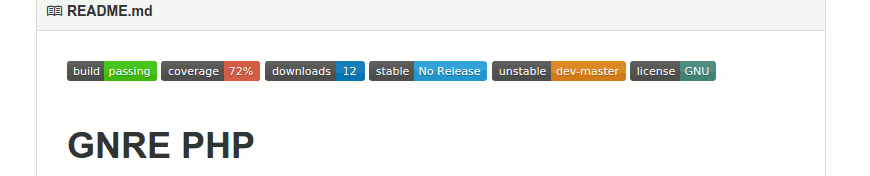
\includegraphics[width=22cm,height=20cm,keepaspectratio=true]{gnrephpbadges}
    }
    \caption{
        Example of Repository Badges \cite{badgeimage}
    }
    \label{gnrephp}
\end{figure}
Badges are small visual images that are usually displayed in a repository's readme file e.g figure \ref{gnrephp}.
Badges display a quantitative metric that indicates a library's inner qualities or aspects that 
can be difficult to access at times. This assists developers with choosing a library
as they can compare and contrast between libraries using badges. These metrics found in the badges
can be dynamically changing over time e.g test code coverage percentage or stay static e.g license information.


\subsection{Online Badge Services}
There are online badge services that exist to help developers use badges for their
repositories without having to create badges from scratch. To get a specific purpose badge,
we would use web services e.g Snyk for security dependency vulnerabilities \cite{snyk} and register
our application with the service to get a full analysis of our project. 
Using the Snyk example, once registered we can add the security GitHub badge to our readme as
suggested in markdown, 
\seqsplit{
[![Known Vulnerabilities](https://snyk.io/test/github/{username}/{repo}/badge.svg)]
(https://snyk.io/test/github/{username}/{repo})}
\cite{snyk}. 
We take our custom project service URL and input its data with the snyk badge svg image itself.


Other services like InchCI for documentation \cite{inchci} or Circleci for build status \cite{circleci} for example
follow a similar method to create a badge. 
However to utilize more badges outside of individual services, Shields.io \cite{shields} is often used
as it is the largest collection
of online hosted repository badges that users can contribute new badges to and use already
existing badges. Just like with individual services, in Shields.io \cite{shields} we would hit custom
http endpoints e.g https://img.shields.io/stackexchange/:stackexchangesite/qm/:query.svg \cite{shields} 
by filling in the 
required query parameters to get the output badge to insert into our repository readme file. 
Users can also use Shields.io \cite{shields} badge templates to customize the image of the badge and 
input their own information into the badge.


\section{Badge Implementation}
\subsection{Overarching Structure of Scripts}

\begin{figure}[!htb]
    \centerline{
        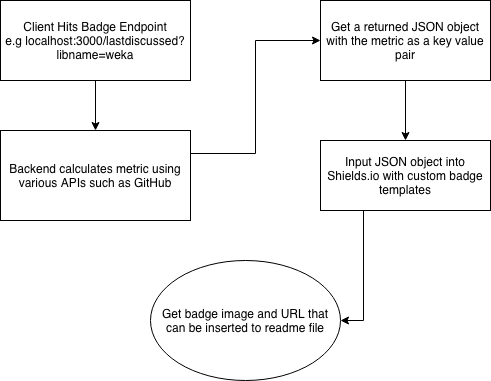
\includegraphics[width=18cm,height=10cm,keepaspectratio=true]{methods}
    }
    \caption{
        Flow diagram representing how we created our badges
    }
    \label{methods}
\end{figure}

Instead of using Shields.io \cite{shields} endpoints, we create our own custom scripts with endpoints 
so that we can prototype our badges locally in a more flexible development environment.
If we were to integrate all the scripts into Shields.io \cite{shieldsrepo} instead of 
developing them locally, we may hit
more extreme cases of run time issues discussed in the limitations section. 
The diagram in figure \ref{methods} represents the flow of how we implement our badges.


\subsection{Security}
\subsubsection{Definition}
The security badge is inspired by Mora's et al. \cite{metrics} security metric implementation.
However, there are limitations related to classifying some security vulnerabilities due to inaccurate
issue descriptions. These inaccuracies would suggest that there was a security problem but in reality was another issue altogether.
To avoid this conflict brought by issue descriptions, 
we propose to use another existing tool called SpotBugs \cite{spotbugs}.
From the SpotBugs \cite{spotbugs} website description itself, the program \textit{uses static analysis to look for bugs in Java code}.
In conjunction with the FindSecBugs \cite{findsecbugs} plugin to provide a larger data set of security bug patterns to look for, 
both these tools will allow for greater accuracy of targeting security bugs.

The security badge represents the number of security bugs reported by SpotBugs \cite{spotbugs} with the FindSecBugs \cite{findsecbugs} plugin.
We filter for only security bug patterns and configure SpotBugs to only classify bugs on the highest confidence setting
with maximum effort toggled on to increase precision. To the user, this badge helps to detect
for any known security vulnerabilities before using the library. 

\subsubsection{Implementation}

\begin{figure}[!htb]
    \centerline{
        
\includegraphics[width=6cm,height=6cm,keepaspectratio=true]{findsecbugsbadge}
    }
    \caption{
        Example of Security Badge
    }
    \label{findsecbugsbadge}
\end{figure}

First, we have a text file that holds open source Java library links hosted on GitHub \cite{github}.
A shell script clones and compiles them respectively under Gradle \cite{gradle} or Maven \cite{maven}.
After compilation, a script runs SpotBugs and FindSecBugs per library under our defined configured settings
and stores the respective result
into the database. The client can hit the security script endpoint to retrieve the saved results which
then can be placed into Shields.io \cite{shields} to output the security badge with an example shown in figure \ref{findsecbugsbadge}. 


\subsection{Last Discussed on Stack Overflow}
\subsubsection{Definition}
We take Mora's et al. \cite{metrics} Last Discussed on Stack Overflow metric and transform it 
into a badge. Based on the metric, the badge represents the latest date of a question posted for a specific
library on the Stack Overflow website \cite{stackoverflow}.
To the user, this badge will display if there is any recent activity using the library and the community
involvement behind it.  

\subsubsection{Implementation}

\begin{figure}[!htb]
    \centerline{
        
\includegraphics[width=10cm,height=10cm,keepaspectratio=true]{lastdiscussedbadge}
    }
    \caption{
        Example of Last Discussed on Stack Overflow Badge
    }
    \label{lastdiscussed}
\end{figure}

Borrowing the implementation technique from Mora et al. \cite{metrics}, we use the StackExchange API \cite{stackexchangeapi}
to search up the library's name under tag search and extract the most popular tag.
With the tag, we make a GET request to the API to search for the most recent question containing the tag
and extract the date. An example of the badge is shown in figure \ref{lastdiscussed}.

\subsection{Issue Response Time}
\subsubsection{Definition}
Using Mora's et al. \cite{metrics} Issue Response Time definition, this badge illustrates the average
amount of days needed to get the first reply to an issue. The badge is calculated via the response time
formula described in \cite{metrics}. It also indicates if there are any changes to the average over time 
as shown by the rightmost symbol in \ref{issueresponse}. 
This badge will allow users to check if there is active maintainence of the library and if there is community support
through the issue discussions. 

\subsubsection{Implementation}

\begin{figure}[!htb]
    \centerline{
        
\includegraphics[width=10cm,height=10cm,keepaspectratio=true]{issueresponsebadge}
    }
    \caption{
        Example of Issue Response Time Badge
    }
    \label{issueresponse}
\end{figure}

We use the algorithm outlined by Mora et al. \cite{metrics} to calculate the issue response time average which
is the difference of all the dates between issue creation date and first comment date over the total number of 
accounted issues. 
The script itself is tweaked to use GitHub's \cite{github} GraphQL API instead of REST to decrease the runtime of iterating through
all the issues and respective comments. The earlier API type allows us to get both the issue creation date and first
comment date in one request call versus the latter API with two calls.
We also discard deleted accounts and do not take them into account in our average.
An example of the badge is shown in figure \ref{issueresponse}.


\subsection{Contributor Pull Request Merge Rate}
\subsubsection{Definition}
Kononenko et al. \cite{shopifyarticle} highlights that, \textit{PRs submitted by the owners are approved more
quicklier compared to those made by external devs}. This can hinder open source development
for developers who wish to partake in the project but are not core maintainers or closely associated with the project.
In addition, there is the lack of assessment defined badges \cite{githubbadges} related to pull requests (PRs)
as of December 2018.
The existing PR badges on Shields.io \cite{shields} display readily available PR information that can be easily found on a 
software repository. Taking both resources \cite{shields, shopifyarticle} into account, this has inspired
the development of the Outside Contributor Pull Request Merge Rate assessment badge. 


The badge represents the percentage of PRs that have been merged into the repository authored by outside contributors.
We define outside contributors using the survey design outlined by Trockman et al. \cite{githubbadges} if they have 
less than 10\% of commits made to a repository. 
This badge helps users to select libraries that are friendly and open to open source contributions,
and easily evaluate the merge rate not accessible beforehand.
With a higher merge rate, it will provide opportunities for developers to extend features of a library with 
higher confidence that their PR will be integrated into the repository.

\subsubsection{Implementation}

\begin{figure}[!htb]
    \centerline{
        
\includegraphics[width=10cm,height=10cm,keepaspectratio=true]{prbadge}
    }
    \caption{
        Example of Outside Contributor PR Merge Rate Badge 
    }
    \label{prbadge}
\end{figure}

We have a seperate script endpoint that uses the GitHub \cite{github} API to get all the users
that have made commits to the library. We classify users as outside contributors or not using
the technique described by Trockman et al. \cite{githubbadges} and store them as a JSON object in the database.
Completing this task will allow us to use another endpoint to calculate the PR metric.
With the GitHub \cite{github} API, we calculate
the average as follows: total number of merged PRs divided by total number of all PRs where 
PRs of all statuses are associated with outside contributors. An example response is shown in figure \ref{prbadge}.


\subsection{Release Frequency}
\subsubsection{Definition}
As defined by Mora et al. \cite{metrics}, release frequency is the average number of days between
releases in repositories. This badge similar to security, pull request, and issue response metrics has 
another visual indicator beside the metric value itself that displays whether or not the average changed over time. 
To the user, the badge suggests if there are fresh releases of software so old code is not being integrated with your
project that can be more vulnerable to bugs and security problems.

\subsubsection{Implementation}

\begin{figure}[!htb]
    \centerline{
        
\includegraphics[width=10cm,height=10cm,keepaspectratio=true]{releasebadge}
    }
    \caption{
        Example of Release Frequency Badge
    }
    \label{releasebadge}
\end{figure}

We use the GitHub \cite{github} API to get all the releases of the library and follow the algorithm
steps outlined by Mora et al. \cite{metrics} to calculate the release frequency metric.
The average is the difference of all the dates between the releases over the total number of releases.
Although not explicitly stated by Mora, we only account for repositories that have two or more releases to compute
the metric. The final result would look similar to the example pictured in figure \ref{releasebadge}.


\section{Evaluation}

\subsection{Open Source Evaluation}

Due to the short timeline of the project, there is no formal evalutation of the work itself.
However, we can qualitatively assess our work by contributing our badges to Shields.io \cite{shields}
and evaluate maintainers thoughts regarding our badges. On the Shields.io Github repository \cite{shieldsrepo}, 
we post an issue \cite{shieldsissue} proposing the addition of the Last Discussed on Stack Overflow badge.
We choose this badge becasuse it has the least amount of data to process and provides us a good indication
if our badge can be successfully integrated into Shields.io \cite{shields} and used by the general public.
A core maintainer responds back highlighting that there are not too many Stack Exchange badges hosted online
and our proposal would be
useful per design changes to be Number of Questions in Past Month on Stack Exchange instead. 
This change would assist in eliminating bias in the metric and skewed data if there is a recent question posted but
for a rarely discussed library confusing a developer using the badge.


\begin{figure}[!htb]
    \centerline{
        
\includegraphics[width=14cm,height=14cm,keepaspectratio=true]{semonthlybadge}
    }
    \caption{
        Example of Stack Exchange Monthly Questions badge
    }
    \label{semonthlybadge}
\end{figure}

In order to make a PR for our proposed badge, we make two other pull requests to respectively
create unit tests for the StackExchange service class and migrate the existing legacy code to Shields.io's newest
API for the service class. This would change the existing StackExchange total questions and StackExchange
user reputation badges. Once completed, we make a PR for the Number of Questions in Past Month on Stack Exchange
badge using the newest Shields.io API. This is calculated by using the StackExchange API and filtering for the 
number of questions between the first and last day of the previous month from today. Having this metric also
allows us to view questions from other StackExchange sub websites besides Stack Overflow.
We were able to successfully get this PR merged and code deployed to the Shields.io \cite{shields} 
production website to be used by the public as displayed in figure \ref{semonthlybadge}. Although we cannot generalize that this can be said
true for the rest of our created badges, this is a good starting evaluation for our badges
that they are indeed useful. 

\subsection{Future Work Evaluation}
If given a longer timeline for this project, posting more GitHub issues for the rest of
our created badges would be a good start. This would allow us to evalutate for more badge design changes
and if they can be successfully pushed to production. Maintainers can comment on our work
and provide an outside opinion on our badges to analyze if our work is suitable. 
In addition, we can determine the amount of users using our StackExchange and other badges as
a metric of popularity to see if users are using our creations. 

\section{Threats to Validity and Limitations}

\subsection{Validity}
\subsubsection{Classification of Outside Contributors}
We use Trockman's et al. \cite{githubbadges} technique to help classify outside contributors for our PR badge.
However, doing some manual testing with our badge with various repositories such
as the Shields.io \cite{shieldsrepo} one, it would misclassify some maintainers as outside contributors.
This would happen if a maintainer has less than 10\% of commits made to a repository which we use as a guideline
for contributors.
To counter this issue in the future, we could iterate through all the commits of a library and define a maintainer as a user who is an explicit 
member of the organization that hosts
the library e.g figure \ref{maintainer} otherwise, the user would be an outside contributor e.g figure \ref{contributor}. 

\begin{figure}[!htb]
    \centerline{
        
\includegraphics[width=14cm,height=14cm,keepaspectratio=true]{maintainer}
    }
    \caption{
        Maintainer Example per posted Shields.io issue \cite{shieldsissue}
    }
    \label{maintainer}
\end{figure}

\begin{figure}[!htb]
    \centerline{
        
\includegraphics[width=14cm,height=14cm,keepaspectratio=true]{contributor}
    }
    \caption{
        Contributor Example per posted Shields.io issue \cite{shieldsissue}
    }
    \label{contributor}
\end{figure}

\subsubsection{Security Bug Classification}
SpotBugs \cite{spotbugs} could end up misclassifying and/or missing security bugs for absent bug patterns.
To make sure our security badge has the most precise value possible, we use SpotBugs \cite{spotbugs}
and FindSecBugs \cite{findsecbugs} on the highest effort and confidence setting to ensure that 
our range of classifcation is wide enough to capture the most number of security vulnerabilities.


\subsection{Limitations}
\subsubsection{Request Timeouts}
Most of the metrics are susceptible to a GitHub \cite{github} image restriction of 3 seconds or less
where the badge has to be displayed before it hits the request timeout limit and not display itself.
To counteract this issue, we made several design decisions per badge to make sure each metric's
run time will be efficient enough to stay within the specified limit.


For the security badge because it takes some time to get the number of bugs from SpotBugs \cite{spotbugs},
we run the shell scripts that runs SpotBugs seperately from the client server interaction to get the metric.
This way when the user hits the security badge endpoint, we only need to return the data previously saved in the 
database from the shell script execution.


For the issue response badge, we return right away to the user the last saved metric saved from the database.
Asynchronously in the background, we calculate the new metric and replace it in the database.
This helps to not block Github from displaying the badge right away and the next time the user hits this endpoint,
we will see the new badge's value.


For the release frequency badge, we determine if the number of releases changed from the last time a user has 
hit this endpoint. If there is no change, we just return the previously saved value which saves a lot of time 
from re-calculating the metric from scratch. If the number of releases changes, we calculate the metric using 
normal means. 


For the PR badge, we calculate the metric starting from the last date a user has hit this specific endpoint.
Caching this date allows us to only need to account for new info starting from the previous script execution
instead of figuring out the metric from scratch for every run.


\subsubsection{Local Scripts}
Currently the scripts to calculate the metrics required for the badges only run
locally on one's own machine. We utilize ngrok
\cite{ngrok} a service that \textit{exposes local servers behind NATS and firewalls to the public
internet over secure tunnels} to help us test our badges online without dealing with the overhead of maintaining
servers and makes it simpler to prototype the badge's functionalities. 
However, this would require restarting ngrok every time after your terminal or machine shuts down
and makes it difficult to keep the ngrok connection alive for others to use because of this limitation.
In the future, deploying our scripts online using services such as Heroku \cite{heroku} or Now \cite{nowjs}
is one possibility. Another solution is to contribute the rest of our badges to Shields.io \cite{shieldsrepo}
and have them hosted there.

\subsubsection{Badge Specific Limitations}
Most limitations of each badge is outlined in the Request Timeouts section.
Specifically for the security badge, there are programming language boundaries.
SpotBugs \cite{spotbugs} itself can only be used for Java libraries and we are 
unable to evaluate the tool's functionalities with other open source libraries written
in different programming languages.


All our badges also depend on the library being open source so that it can openly
access required information without deadling with authentication and privacy concerns.

\section{Conclusion and Future Work}
% Future work
% Host Scripts openly using something like heroku or now.js
% Improve Error handling to make sure client knows any bad http codes
% make front end application to display these metrics to get detailed info, visualizations of metrics
% being used where and number of people suing them in line graph


\newpage
\bibliographystyle{IEEEtran}
\bibliography{bibliography}
\end{document}